% Created by tikzDevice version 0.12.6 on 2026-08-08 13:32:30
% !TEX encoding = UTF-8 Unicode
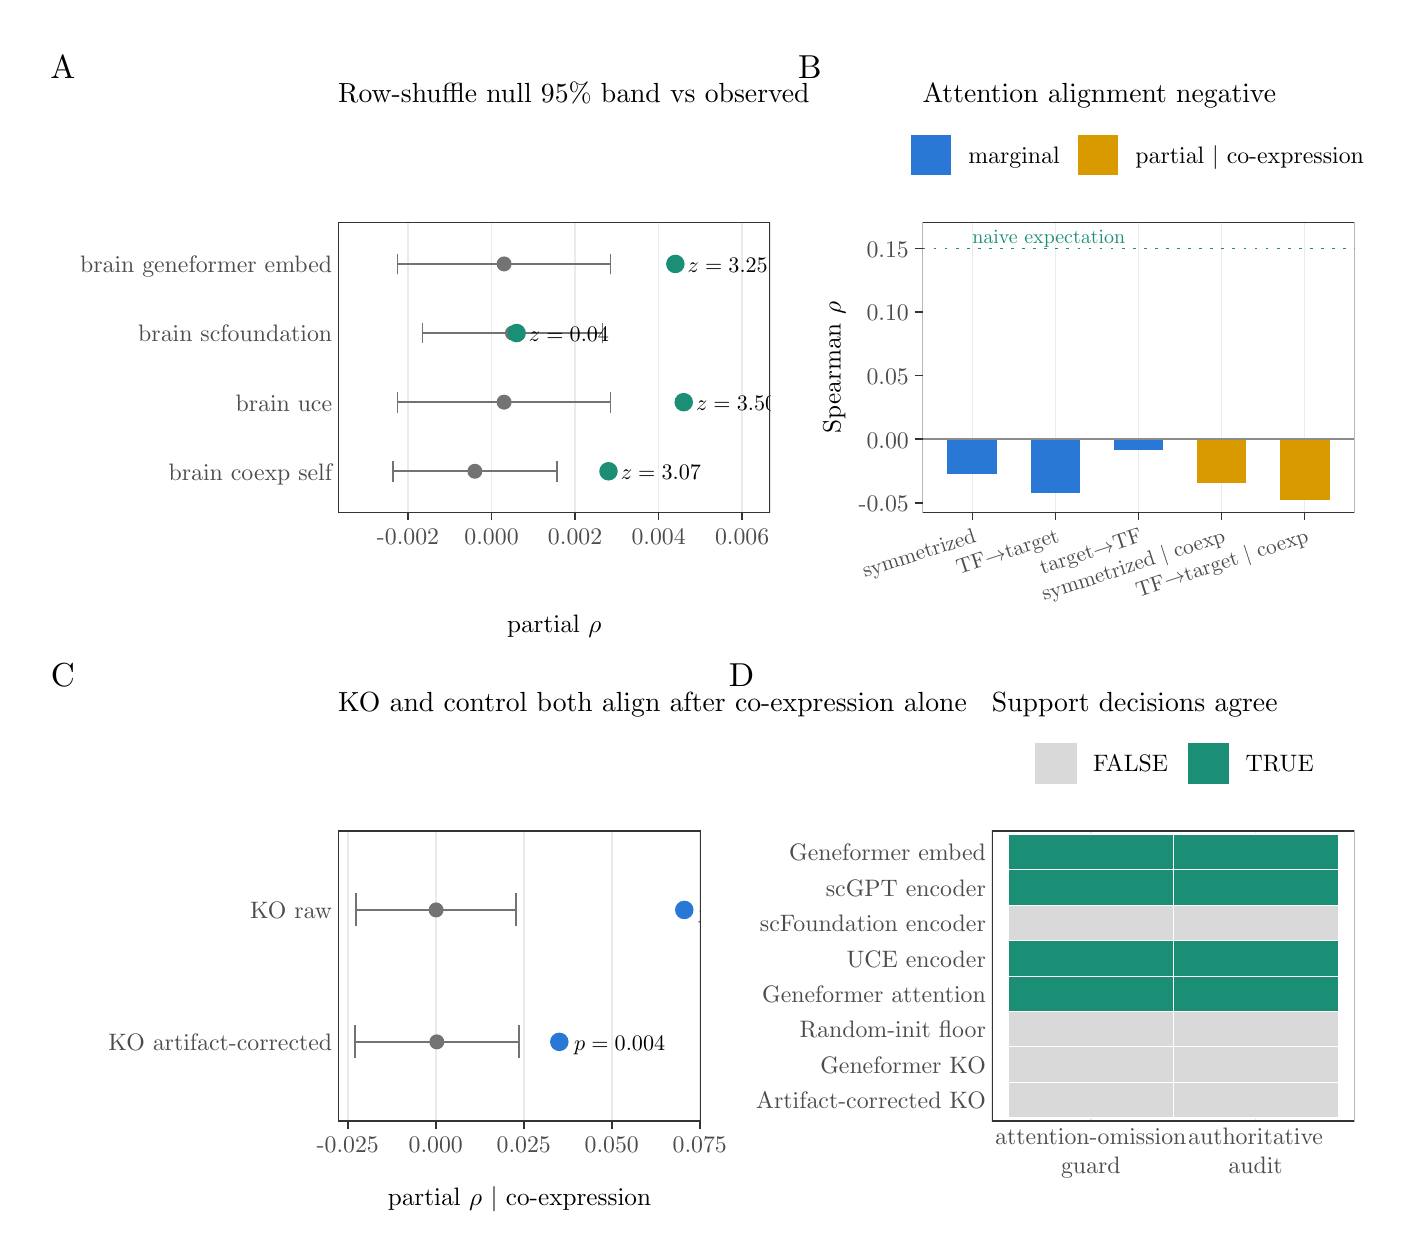
\begin{tikzpicture}[x=1pt,y=1pt]
\definecolor{fillColor}{RGB}{255,255,255}
\path[use as bounding box,fill=fillColor,fill opacity=0.00] (0,0) rectangle (491.44,433.62);
\begin{scope}
\path[clip] (  0.00,  0.00) rectangle (491.44,433.62);
\definecolor{drawColor}{RGB}{255,255,255}
\definecolor{fillColor}{RGB}{255,255,255}

\path[draw=drawColor,line width= 0.6pt,line join=round,line cap=round,fill=fillColor] ( -0.00,  0.00) rectangle (491.44,433.62);
\end{scope}
\begin{scope}
\path[clip] (  4.00,209.82) rectangle (274.30,429.62);
\definecolor{drawColor}{RGB}{255,255,255}
\definecolor{fillColor}{RGB}{255,255,255}

\path[draw=drawColor,line width= 0.6pt,line join=round,line cap=round,fill=fillColor] (  4.00,209.82) rectangle (274.30,429.62);
\end{scope}
\begin{scope}
\path[clip] (274.30,209.82) rectangle (485.44,429.62);
\definecolor{drawColor}{RGB}{255,255,255}
\definecolor{fillColor}{RGB}{255,255,255}

\path[draw=drawColor,line width= 0.6pt,line join=round,line cap=round,fill=fillColor] (274.30,209.82) rectangle (485.44,429.62);
\end{scope}
\begin{scope}
\path[clip] (112.22,258.34) rectangle (268.30,363.22);
\definecolor{fillColor}{RGB}{255,255,255}

\path[fill=fillColor] (112.22,258.34) rectangle (268.30,363.22);
\definecolor{drawColor}{gray}{0.92}

\path[draw=drawColor,line width= 0.6pt,line join=round] (137.43,258.34) --
	(137.43,363.22);

\path[draw=drawColor,line width= 0.6pt,line join=round] (167.62,258.34) --
	(167.62,363.22);

\path[draw=drawColor,line width= 0.6pt,line join=round] (197.81,258.34) --
	(197.81,363.22);

\path[draw=drawColor,line width= 0.6pt,line join=round] (228.00,258.34) --
	(228.00,363.22);

\path[draw=drawColor,line width= 0.6pt,line join=round] (258.19,258.34) --
	(258.19,363.22);
\definecolor{drawColor}{gray}{0.45}

\path[draw=drawColor,line width= 0.6pt,line join=round] (210.61,344.49) --
	(210.61,351.98);

\path[draw=drawColor,line width= 0.6pt,line join=round] (210.61,348.24) --
	(133.68,348.24);

\path[draw=drawColor,line width= 0.6pt,line join=round] (133.68,344.49) --
	(133.68,351.98);

\path[draw=drawColor,line width= 0.6pt,line join=round] (207.71,319.52) --
	(207.71,327.01);

\path[draw=drawColor,line width= 0.6pt,line join=round] (207.71,323.26) --
	(142.62,323.26);

\path[draw=drawColor,line width= 0.6pt,line join=round] (142.62,319.52) --
	(142.62,327.01);

\path[draw=drawColor,line width= 0.6pt,line join=round] (210.61,294.55) --
	(210.61,302.04);

\path[draw=drawColor,line width= 0.6pt,line join=round] (210.61,298.29) --
	(133.68,298.29);

\path[draw=drawColor,line width= 0.6pt,line join=round] (133.68,294.55) --
	(133.68,302.04);

\path[draw=drawColor,line width= 0.6pt,line join=round] (191.17,269.57) --
	(191.17,277.07);

\path[draw=drawColor,line width= 0.6pt,line join=round] (191.17,273.32) --
	(131.99,273.32);

\path[draw=drawColor,line width= 0.6pt,line join=round] (131.99,269.57) --
	(131.99,277.07);
\definecolor{fillColor}{gray}{0.45}

\path[draw=drawColor,line width= 0.4pt,line join=round,line cap=round,fill=fillColor] (172.15,348.24) circle (  2.50);

\path[draw=drawColor,line width= 0.4pt,line join=round,line cap=round,fill=fillColor] (175.17,323.26) circle (  2.50);

\path[draw=drawColor,line width= 0.4pt,line join=round,line cap=round,fill=fillColor] (172.15,298.29) circle (  2.50);

\path[draw=drawColor,line width= 0.4pt,line join=round,line cap=round,fill=fillColor] (161.58,273.32) circle (  2.50);
\definecolor{drawColor}{RGB}{27,143,117}
\definecolor{fillColor}{RGB}{27,143,117}

\path[draw=drawColor,line width= 0.4pt,line join=round,line cap=round,fill=fillColor] (234.04,348.24) circle (  3.14);

\path[draw=drawColor,line width= 0.4pt,line join=round,line cap=round,fill=fillColor] (176.68,323.26) circle (  3.14);

\path[draw=drawColor,line width= 0.4pt,line join=round,line cap=round,fill=fillColor] (237.06,298.29) circle (  3.14);

\path[draw=drawColor,line width= 0.4pt,line join=round,line cap=round,fill=fillColor] (209.88,273.32) circle (  3.14);
\definecolor{drawColor}{RGB}{0,0,0}

\node[text=drawColor,anchor=base west,inner sep=0pt, outer sep=0pt, scale=  0.80] at (238.48,345.27) {$z=3.25$};

\node[text=drawColor,anchor=base west,inner sep=0pt, outer sep=0pt, scale=  0.80] at (181.12,320.30) {$z=0.04$};

\node[text=drawColor,anchor=base west,inner sep=0pt, outer sep=0pt, scale=  0.80] at (241.50,295.32) {$z=3.50$};

\node[text=drawColor,anchor=base west,inner sep=0pt, outer sep=0pt, scale=  0.80] at (214.33,270.35) {$z=3.07$};
\definecolor{drawColor}{gray}{0.20}

\path[draw=drawColor,line width= 0.6pt,line join=round,line cap=round] (112.22,258.34) rectangle (268.30,363.22);
\end{scope}
\begin{scope}
\path[clip] (  0.00,  0.00) rectangle (491.44,433.62);
\definecolor{drawColor}{gray}{0.30}

\node[text=drawColor,anchor=base east,inner sep=0pt, outer sep=0pt, scale=  0.86] at (110.02,270.12) {brain coexp self};

\node[text=drawColor,anchor=base east,inner sep=0pt, outer sep=0pt, scale=  0.86] at (110.02,295.10) {brain uce};

\node[text=drawColor,anchor=base east,inner sep=0pt, outer sep=0pt, scale=  0.86] at (110.02,320.07) {brain scfoundation};

\node[text=drawColor,anchor=base east,inner sep=0pt, outer sep=0pt, scale=  0.86] at (110.02,345.04) {brain geneformer embed};
\end{scope}
\begin{scope}
\path[clip] (  0.00,  0.00) rectangle (491.44,433.62);
\definecolor{drawColor}{gray}{0.20}

\path[draw=drawColor,line width= 0.6pt,line join=round] (137.43,255.59) --
	(137.43,258.34);

\path[draw=drawColor,line width= 0.6pt,line join=round] (167.62,255.59) --
	(167.62,258.34);

\path[draw=drawColor,line width= 0.6pt,line join=round] (197.81,255.59) --
	(197.81,258.34);

\path[draw=drawColor,line width= 0.6pt,line join=round] (228.00,255.59) --
	(228.00,258.34);

\path[draw=drawColor,line width= 0.6pt,line join=round] (258.19,255.59) --
	(258.19,258.34);
\end{scope}
\begin{scope}
\path[clip] (  0.00,  0.00) rectangle (491.44,433.62);
\definecolor{drawColor}{gray}{0.30}

\node[text=drawColor,anchor=base,inner sep=0pt, outer sep=0pt, scale=  0.86] at (137.43,246.99) {-0.002};

\node[text=drawColor,anchor=base,inner sep=0pt, outer sep=0pt, scale=  0.86] at (167.62,246.99) {0.000};

\node[text=drawColor,anchor=base,inner sep=0pt, outer sep=0pt, scale=  0.86] at (197.81,246.99) {0.002};

\node[text=drawColor,anchor=base,inner sep=0pt, outer sep=0pt, scale=  0.86] at (228.00,246.99) {0.004};

\node[text=drawColor,anchor=base,inner sep=0pt, outer sep=0pt, scale=  0.86] at (258.19,246.99) {0.006};
\end{scope}
\begin{scope}
\path[clip] (  0.00,  0.00) rectangle (491.44,433.62);
\definecolor{drawColor}{RGB}{0,0,0}

\node[text=drawColor,anchor=base,inner sep=0pt, outer sep=0pt, scale=  0.91] at (190.26,214.97) {partial $\rho$};
\end{scope}
\begin{scope}
\path[clip] (  0.00,  0.00) rectangle (491.44,433.62);
\definecolor{drawColor}{RGB}{0,0,0}

\node[text=drawColor,anchor=base west,inner sep=0pt, outer sep=0pt, scale=  1.00] at (112.22,406.49) {Row-shuffle null 95\% band vs observed};
\end{scope}
\begin{scope}
\path[clip] (  0.00,  0.00) rectangle (491.44,433.62);
\definecolor{drawColor}{RGB}{0,0,0}

\node[text=drawColor,anchor=base,inner sep=0pt, outer sep=0pt, scale=  1.20] at ( 12.74,415.32) {A};
\end{scope}
\begin{scope}
\path[clip] (323.35,258.34) rectangle (479.44,363.22);
\definecolor{fillColor}{RGB}{255,255,255}

\path[fill=fillColor] (323.35,258.34) rectangle (479.44,363.22);
\definecolor{drawColor}{gray}{0.92}

\path[draw=drawColor,line width= 0.6pt,line join=round] (341.36,258.34) --
	(341.36,363.22);

\path[draw=drawColor,line width= 0.6pt,line join=round] (371.38,258.34) --
	(371.38,363.22);

\path[draw=drawColor,line width= 0.6pt,line join=round] (401.39,258.34) --
	(401.39,363.22);

\path[draw=drawColor,line width= 0.6pt,line join=round] (431.41,258.34) --
	(431.41,363.22);

\path[draw=drawColor,line width= 0.6pt,line join=round] (461.43,258.34) --
	(461.43,363.22);
\definecolor{fillColor}{RGB}{42,120,214}

\path[fill=fillColor] (332.36,272.43) rectangle (350.37,284.93);

\path[fill=fillColor] (362.37,265.36) rectangle (380.38,284.93);

\path[fill=fillColor] (392.39,280.93) rectangle (410.40,284.93);
\definecolor{fillColor}{RGB}{217,154,0}

\path[fill=fillColor] (422.40,268.99) rectangle (440.41,284.93);

\path[fill=fillColor] (452.42,263.10) rectangle (470.43,284.93);
\definecolor{drawColor}{gray}{0.55}

\path[draw=drawColor,line width= 0.6pt,line join=round] (323.35,284.93) -- (479.44,284.93);
\definecolor{drawColor}{RGB}{27,143,117}

\path[draw=drawColor,line width= 0.3pt,dash pattern=on 1pt off 3pt ,line join=round] (323.35,353.86) -- (479.44,353.86);

\node[text=drawColor,anchor=base west,inner sep=0pt, outer sep=0pt, scale=  0.72] at (341.36,355.77) {naive expectation};
\definecolor{drawColor}{gray}{0.20}

\path[draw=drawColor,line width= 0.6pt,line join=round,line cap=round] (323.35,258.34) rectangle (479.44,363.22);
\end{scope}
\begin{scope}
\path[clip] (  0.00,  0.00) rectangle (491.44,433.62);
\definecolor{drawColor}{gray}{0.30}

\node[text=drawColor,anchor=base east,inner sep=0pt, outer sep=0pt, scale=  0.86] at (318.40,258.76) {-0.05};

\node[text=drawColor,anchor=base east,inner sep=0pt, outer sep=0pt, scale=  0.86] at (318.40,281.73) {0.00};

\node[text=drawColor,anchor=base east,inner sep=0pt, outer sep=0pt, scale=  0.86] at (318.40,304.71) {0.05};

\node[text=drawColor,anchor=base east,inner sep=0pt, outer sep=0pt, scale=  0.86] at (318.40,327.69) {0.10};

\node[text=drawColor,anchor=base east,inner sep=0pt, outer sep=0pt, scale=  0.86] at (318.40,350.66) {0.15};
\end{scope}
\begin{scope}
\path[clip] (  0.00,  0.00) rectangle (491.44,433.62);
\definecolor{drawColor}{gray}{0.20}

\path[draw=drawColor,line width= 0.6pt,line join=round] (320.60,261.95) --
	(323.35,261.95);

\path[draw=drawColor,line width= 0.6pt,line join=round] (320.60,284.93) --
	(323.35,284.93);

\path[draw=drawColor,line width= 0.6pt,line join=round] (320.60,307.91) --
	(323.35,307.91);

\path[draw=drawColor,line width= 0.6pt,line join=round] (320.60,330.88) --
	(323.35,330.88);

\path[draw=drawColor,line width= 0.6pt,line join=round] (320.60,353.86) --
	(323.35,353.86);
\end{scope}
\begin{scope}
\path[clip] (  0.00,  0.00) rectangle (491.44,433.62);
\definecolor{drawColor}{gray}{0.20}

\path[draw=drawColor,line width= 0.6pt,line join=round] (341.36,255.59) --
	(341.36,258.34);

\path[draw=drawColor,line width= 0.6pt,line join=round] (371.38,255.59) --
	(371.38,258.34);

\path[draw=drawColor,line width= 0.6pt,line join=round] (401.39,255.59) --
	(401.39,258.34);

\path[draw=drawColor,line width= 0.6pt,line join=round] (431.41,255.59) --
	(431.41,258.34);

\path[draw=drawColor,line width= 0.6pt,line join=round] (461.43,255.59) --
	(461.43,258.34);
\end{scope}
\begin{scope}
\path[clip] (  0.00,  0.00) rectangle (491.44,433.62);
\definecolor{drawColor}{gray}{0.30}

\node[text=drawColor,rotate= 18.00,anchor=base east,inner sep=0pt, outer sep=0pt, scale=  0.77] at (343.13,247.95) {symmetrized};

\node[text=drawColor,rotate= 18.00,anchor=base east,inner sep=0pt, outer sep=0pt, scale=  0.77] at (373.14,247.95) {TF$\to$target};

\node[text=drawColor,rotate= 18.00,anchor=base east,inner sep=0pt, outer sep=0pt, scale=  0.77] at (403.16,247.95) {target$\to$TF};

\node[text=drawColor,rotate= 18.00,anchor=base east,inner sep=0pt, outer sep=0pt, scale=  0.77] at (433.18,247.95) {symmetrized $|$ coexp};

\node[text=drawColor,rotate= 18.00,anchor=base east,inner sep=0pt, outer sep=0pt, scale=  0.77] at (463.19,247.95) {TF$\to$target $|$ coexp};
\end{scope}
\begin{scope}
\path[clip] (  0.00,  0.00) rectangle (491.44,433.62);
\definecolor{drawColor}{RGB}{0,0,0}

\node[text=drawColor,rotate= 90.00,anchor=base,inner sep=0pt, outer sep=0pt, scale=  0.91] at (293.80,310.78) {Spearman $\rho$};
\end{scope}
\begin{scope}
\path[clip] (  0.00,  0.00) rectangle (491.44,433.62);
\definecolor{fillColor}{RGB}{255,255,255}

\path[fill=fillColor] (313.02,374.22) rectangle (489.76,401.12);
\end{scope}
\begin{scope}
\path[clip] (  0.00,  0.00) rectangle (491.44,433.62);
\definecolor{fillColor}{RGB}{255,255,255}

\path[fill=fillColor] (318.52,379.72) rectangle (334.42,395.62);
\definecolor{fillColor}{RGB}{42,120,214}

\path[fill=fillColor] (319.24,380.43) rectangle (333.71,394.91);
\end{scope}
\begin{scope}
\path[clip] (  0.00,  0.00) rectangle (491.44,433.62);
\definecolor{fillColor}{RGB}{255,255,255}

\path[fill=fillColor] (378.90,379.72) rectangle (394.80,395.62);
\definecolor{fillColor}{RGB}{217,154,0}

\path[fill=fillColor] (379.61,380.43) rectangle (394.09,394.91);
\end{scope}
\begin{scope}
\path[clip] (  0.00,  0.00) rectangle (491.44,433.62);
\definecolor{drawColor}{RGB}{0,0,0}

\node[text=drawColor,anchor=base west,inner sep=0pt, outer sep=0pt, scale=  0.86] at (339.92,384.47) {marginal};
\end{scope}
\begin{scope}
\path[clip] (  0.00,  0.00) rectangle (491.44,433.62);
\definecolor{drawColor}{RGB}{0,0,0}

\node[text=drawColor,anchor=base west,inner sep=0pt, outer sep=0pt, scale=  0.86] at (400.30,384.47) {partial $|$ co-expression};
\end{scope}
\begin{scope}
\path[clip] (  0.00,  0.00) rectangle (491.44,433.62);
\definecolor{drawColor}{RGB}{0,0,0}

\node[text=drawColor,anchor=base west,inner sep=0pt, outer sep=0pt, scale=  1.00] at (323.35,406.49) {Attention alignment negative};
\end{scope}
\begin{scope}
\path[clip] (  0.00,  0.00) rectangle (491.44,433.62);
\definecolor{drawColor}{RGB}{0,0,0}

\node[text=drawColor,anchor=base,inner sep=0pt, outer sep=0pt, scale=  1.20] at (282.69,415.32) {B};
\end{scope}
\begin{scope}
\path[clip] (  4.00,  3.00) rectangle (249.22,209.82);
\definecolor{drawColor}{RGB}{255,255,255}
\definecolor{fillColor}{RGB}{255,255,255}

\path[draw=drawColor,line width= 0.6pt,line join=round,line cap=round,fill=fillColor] (  4.00,  3.00) rectangle (249.22,209.82);
\end{scope}
\begin{scope}
\path[clip] (249.22,  3.00) rectangle (485.44,209.82);
\definecolor{drawColor}{RGB}{255,255,255}
\definecolor{fillColor}{RGB}{255,255,255}

\path[draw=drawColor,line width= 0.6pt,line join=round,line cap=round,fill=fillColor] (249.22,  3.00) rectangle (485.44,209.82);
\end{scope}
\begin{scope}
\path[clip] (112.22, 38.53) rectangle (243.22,143.42);
\definecolor{fillColor}{RGB}{255,255,255}

\path[fill=fillColor] (112.22, 38.53) rectangle (243.22,143.42);
\definecolor{drawColor}{gray}{0.92}

\path[draw=drawColor,line width= 0.6pt,line join=round] (115.66, 38.53) --
	(115.66,143.42);

\path[draw=drawColor,line width= 0.6pt,line join=round] (147.46, 38.53) --
	(147.46,143.42);

\path[draw=drawColor,line width= 0.6pt,line join=round] (179.26, 38.53) --
	(179.26,143.42);

\path[draw=drawColor,line width= 0.6pt,line join=round] (211.06, 38.53) --
	(211.06,143.42);

\path[draw=drawColor,line width= 0.6pt,line join=round] (242.87, 38.53) --
	(242.87,143.42);
\definecolor{drawColor}{gray}{0.45}

\path[draw=drawColor,line width= 0.6pt,line join=round] (176.51,108.85) --
	(176.51,120.77);

\path[draw=drawColor,line width= 0.6pt,line join=round] (176.51,114.81) --
	(118.67,114.81);

\path[draw=drawColor,line width= 0.6pt,line join=round] (118.67,108.85) --
	(118.67,120.77);

\path[draw=drawColor,line width= 0.6pt,line join=round] (177.51, 61.18) --
	(177.51, 73.10);

\path[draw=drawColor,line width= 0.6pt,line join=round] (177.51, 67.14) --
	(118.17, 67.14);

\path[draw=drawColor,line width= 0.6pt,line join=round] (118.17, 61.18) --
	(118.17, 73.10);
\definecolor{fillColor}{gray}{0.45}

\path[draw=drawColor,line width= 0.4pt,line join=round,line cap=round,fill=fillColor] (147.59,114.81) circle (  2.50);

\path[draw=drawColor,line width= 0.4pt,line join=round,line cap=round,fill=fillColor] (147.84, 67.14) circle (  2.50);
\definecolor{drawColor}{RGB}{42,120,214}
\definecolor{fillColor}{RGB}{42,120,214}

\path[draw=drawColor,line width= 0.4pt,line join=round,line cap=round,fill=fillColor] (237.27,114.81) circle (  3.14);

\path[draw=drawColor,line width= 0.4pt,line join=round,line cap=round,fill=fillColor] (192.11, 67.14) circle (  3.14);
\definecolor{drawColor}{RGB}{0,0,0}

\node[text=drawColor,anchor=base west,inner sep=0pt, outer sep=0pt, scale=  0.80] at (242.59,111.85) {$p=0.001$};

\node[text=drawColor,anchor=base west,inner sep=0pt, outer sep=0pt, scale=  0.80] at (197.44, 64.17) {$p=0.004$};
\definecolor{drawColor}{gray}{0.20}

\path[draw=drawColor,line width= 0.6pt,line join=round,line cap=round] (112.22, 38.53) rectangle (243.22,143.42);
\end{scope}
\begin{scope}
\path[clip] (  0.00,  0.00) rectangle (491.44,433.62);
\definecolor{drawColor}{gray}{0.30}

\node[text=drawColor,anchor=base east,inner sep=0pt, outer sep=0pt, scale=  0.86] at (110.02, 63.94) {KO artifact-corrected};

\node[text=drawColor,anchor=base east,inner sep=0pt, outer sep=0pt, scale=  0.86] at (110.02,111.62) {KO raw};
\end{scope}
\begin{scope}
\path[clip] (  0.00,  0.00) rectangle (491.44,433.62);
\definecolor{drawColor}{gray}{0.20}

\path[draw=drawColor,line width= 0.6pt,line join=round] (115.66, 35.78) --
	(115.66, 38.53);

\path[draw=drawColor,line width= 0.6pt,line join=round] (147.46, 35.78) --
	(147.46, 38.53);

\path[draw=drawColor,line width= 0.6pt,line join=round] (179.26, 35.78) --
	(179.26, 38.53);

\path[draw=drawColor,line width= 0.6pt,line join=round] (211.06, 35.78) --
	(211.06, 38.53);

\path[draw=drawColor,line width= 0.6pt,line join=round] (242.87, 35.78) --
	(242.87, 38.53);
\end{scope}
\begin{scope}
\path[clip] (  0.00,  0.00) rectangle (491.44,433.62);
\definecolor{drawColor}{gray}{0.30}

\node[text=drawColor,anchor=base,inner sep=0pt, outer sep=0pt, scale=  0.86] at (115.66, 27.19) {-0.025};

\node[text=drawColor,anchor=base,inner sep=0pt, outer sep=0pt, scale=  0.86] at (147.46, 27.19) {0.000};

\node[text=drawColor,anchor=base,inner sep=0pt, outer sep=0pt, scale=  0.86] at (179.26, 27.19) {0.025};

\node[text=drawColor,anchor=base,inner sep=0pt, outer sep=0pt, scale=  0.86] at (211.06, 27.19) {0.050};

\node[text=drawColor,anchor=base,inner sep=0pt, outer sep=0pt, scale=  0.86] at (242.87, 27.19) {0.075};
\end{scope}
\begin{scope}
\path[clip] (  0.00,  0.00) rectangle (491.44,433.62);
\definecolor{drawColor}{RGB}{0,0,0}

\node[text=drawColor,anchor=base,inner sep=0pt, outer sep=0pt, scale=  0.91] at (177.72,  8.16) {partial $\rho$ $|$ co-expression};
\end{scope}
\begin{scope}
\path[clip] (  0.00,  0.00) rectangle (491.44,433.62);
\definecolor{drawColor}{RGB}{0,0,0}

\node[text=drawColor,anchor=base west,inner sep=0pt, outer sep=0pt, scale=  1.00] at (112.22,186.69) {KO and control both align after co-expression alone};
\end{scope}
\begin{scope}
\path[clip] (  0.00,  0.00) rectangle (491.44,433.62);
\definecolor{drawColor}{RGB}{0,0,0}

\node[text=drawColor,anchor=base,inner sep=0pt, outer sep=0pt, scale=  1.20] at ( 12.74,195.51) {C};
\end{scope}
\begin{scope}
\path[clip] (348.43, 38.53) rectangle (479.44,143.42);
\definecolor{fillColor}{RGB}{255,255,255}

\path[fill=fillColor] (348.43, 38.53) rectangle (479.44,143.42);
\definecolor{drawColor}{gray}{0.92}

\path[draw=drawColor,line width= 0.6pt,line join=round] (384.16, 38.53) --
	(384.16,143.42);

\path[draw=drawColor,line width= 0.6pt,line join=round] (443.71, 38.53) --
	(443.71,143.42);
\definecolor{drawColor}{RGB}{255,255,255}
\definecolor{fillColor}{RGB}{27,143,117}

\path[draw=drawColor,line width= 0.2pt,fill=fillColor] (413.93,129.35) rectangle (473.48,142.14);

\path[draw=drawColor,line width= 0.2pt,fill=fillColor] (413.93,116.56) rectangle (473.48,129.35);
\definecolor{fillColor}{gray}{0.85}

\path[draw=drawColor,line width= 0.2pt,fill=fillColor] (413.93,103.77) rectangle (473.48,116.56);
\definecolor{fillColor}{RGB}{27,143,117}

\path[draw=drawColor,line width= 0.2pt,fill=fillColor] (413.93, 90.98) rectangle (473.48,103.77);

\path[draw=drawColor,line width= 0.2pt,fill=fillColor] (413.93, 78.19) rectangle (473.48, 90.98);
\definecolor{fillColor}{gray}{0.85}

\path[draw=drawColor,line width= 0.2pt,fill=fillColor] (413.93, 65.39) rectangle (473.48, 78.19);

\path[draw=drawColor,line width= 0.2pt,fill=fillColor] (413.93, 52.60) rectangle (473.48, 65.39);

\path[draw=drawColor,line width= 0.2pt,fill=fillColor] (413.93, 39.81) rectangle (473.48, 52.60);
\definecolor{fillColor}{RGB}{27,143,117}

\path[draw=drawColor,line width= 0.2pt,fill=fillColor] (354.38,129.35) rectangle (413.93,142.14);

\path[draw=drawColor,line width= 0.2pt,fill=fillColor] (354.38,116.56) rectangle (413.93,129.35);
\definecolor{fillColor}{gray}{0.85}

\path[draw=drawColor,line width= 0.2pt,fill=fillColor] (354.38,103.77) rectangle (413.93,116.56);
\definecolor{fillColor}{RGB}{27,143,117}

\path[draw=drawColor,line width= 0.2pt,fill=fillColor] (354.38, 90.98) rectangle (413.93,103.77);

\path[draw=drawColor,line width= 0.2pt,fill=fillColor] (354.38, 78.19) rectangle (413.93, 90.98);
\definecolor{fillColor}{gray}{0.85}

\path[draw=drawColor,line width= 0.2pt,fill=fillColor] (354.38, 65.39) rectangle (413.93, 78.19);

\path[draw=drawColor,line width= 0.2pt,fill=fillColor] (354.38, 52.60) rectangle (413.93, 65.39);

\path[draw=drawColor,line width= 0.2pt,fill=fillColor] (354.38, 39.81) rectangle (413.93, 52.60);
\definecolor{drawColor}{gray}{0.20}

\path[draw=drawColor,line width= 0.6pt,line join=round,line cap=round] (348.43, 38.53) rectangle (479.44,143.42);
\end{scope}
\begin{scope}
\path[clip] (  0.00,  0.00) rectangle (491.44,433.62);
\definecolor{drawColor}{gray}{0.30}

\node[text=drawColor,anchor=base east,inner sep=0pt, outer sep=0pt, scale=  0.86] at (346.23, 43.01) {Artifact-corrected KO};

\node[text=drawColor,anchor=base east,inner sep=0pt, outer sep=0pt, scale=  0.86] at (346.23, 55.80) {Geneformer KO};

\node[text=drawColor,anchor=base east,inner sep=0pt, outer sep=0pt, scale=  0.86] at (346.23, 68.59) {Random-init floor};

\node[text=drawColor,anchor=base east,inner sep=0pt, outer sep=0pt, scale=  0.86] at (346.23, 81.38) {Geneformer attention};

\node[text=drawColor,anchor=base east,inner sep=0pt, outer sep=0pt, scale=  0.86] at (346.23, 94.18) {UCE encoder};

\node[text=drawColor,anchor=base east,inner sep=0pt, outer sep=0pt, scale=  0.86] at (346.23,106.97) {scFoundation encoder};

\node[text=drawColor,anchor=base east,inner sep=0pt, outer sep=0pt, scale=  0.86] at (346.23,119.76) {scGPT encoder};

\node[text=drawColor,anchor=base east,inner sep=0pt, outer sep=0pt, scale=  0.86] at (346.23,132.55) {Geneformer embed};
\end{scope}
\begin{scope}
\path[clip] (  0.00,  0.00) rectangle (491.44,433.62);
\definecolor{drawColor}{gray}{0.30}

\node[text=drawColor,anchor=base,inner sep=0pt, outer sep=0pt, scale=  0.86] at (384.16, 29.94) {attention-omission};

\node[text=drawColor,anchor=base,inner sep=0pt, outer sep=0pt, scale=  0.86] at (384.16, 19.68) {guard};

\node[text=drawColor,anchor=base,inner sep=0pt, outer sep=0pt, scale=  0.86] at (443.71, 29.94) {authoritative};

\node[text=drawColor,anchor=base,inner sep=0pt, outer sep=0pt, scale=  0.86] at (443.71, 19.68) {audit};
\end{scope}
\begin{scope}
\path[clip] (  0.00,  0.00) rectangle (491.44,433.62);
\definecolor{fillColor}{RGB}{255,255,255}

\path[fill=fillColor] (358.08,154.42) rectangle (469.79,181.32);
\end{scope}
\begin{scope}
\path[clip] (  0.00,  0.00) rectangle (491.44,433.62);
\definecolor{fillColor}{RGB}{255,255,255}

\path[fill=fillColor] (363.58,159.92) rectangle (379.48,175.82);
\definecolor{drawColor}{RGB}{255,255,255}
\definecolor{fillColor}{gray}{0.85}

\path[draw=drawColor,line width= 0.2pt,fill=fillColor] (363.86,160.20) rectangle (379.19,175.53);
\end{scope}
\begin{scope}
\path[clip] (  0.00,  0.00) rectangle (491.44,433.62);
\definecolor{fillColor}{RGB}{255,255,255}

\path[fill=fillColor] (418.72,159.92) rectangle (434.62,175.82);
\definecolor{drawColor}{RGB}{255,255,255}
\definecolor{fillColor}{RGB}{27,143,117}

\path[draw=drawColor,line width= 0.2pt,fill=fillColor] (419.00,160.20) rectangle (434.33,175.53);
\end{scope}
\begin{scope}
\path[clip] (  0.00,  0.00) rectangle (491.44,433.62);
\definecolor{drawColor}{RGB}{0,0,0}

\node[text=drawColor,anchor=base west,inner sep=0pt, outer sep=0pt, scale=  0.86] at (384.98,164.67) {FALSE};
\end{scope}
\begin{scope}
\path[clip] (  0.00,  0.00) rectangle (491.44,433.62);
\definecolor{drawColor}{RGB}{0,0,0}

\node[text=drawColor,anchor=base west,inner sep=0pt, outer sep=0pt, scale=  0.86] at (440.12,164.67) {TRUE};
\end{scope}
\begin{scope}
\path[clip] (  0.00,  0.00) rectangle (491.44,433.62);
\definecolor{drawColor}{RGB}{0,0,0}

\node[text=drawColor,anchor=base west,inner sep=0pt, outer sep=0pt, scale=  1.00] at (348.43,186.69) {Support decisions agree};
\end{scope}
\begin{scope}
\path[clip] (  0.00,  0.00) rectangle (491.44,433.62);
\definecolor{drawColor}{RGB}{0,0,0}

\node[text=drawColor,anchor=base,inner sep=0pt, outer sep=0pt, scale=  1.20] at (257.97,195.51) {D};
\end{scope}
\end{tikzpicture}
